\mychapter{3}{Opis riešenia - Server manažmentu rolí a používateľov}


%ked vyhladavam užívateľov, nemal by som dať limit... aj ked to mi neotestujú :D
\section{Určenie požiadaviek}
Aplikačným výstupom tejto bakalárskej práce je web stránka, ktorej účelom je vytvoriť jednoduché a intuitívne aplikačné rozhranie pre priraďovanie používateľov k roliam. V aplikácii by sa mali dať vyhľadať všetci používatelia vo firme. Pre rýchlejšie vyhľadávanie a prehľadné údaje bude možné používateľov zotriediť do kategórie podľa rolí. Užívatelia, ktorí nemajú priradenú žiadnu rolu, budú mať vlastnú podsekciu. Vďaka tomu bude mať firma každého používateľa pod kontrolou, aby mal priradenú minimálne jednu rolu. Užívatelia sa budú dať zoradiť podľa ich id, mena, priezviska alebo e-mailovej adresy. V každej podsekcii umožníme vyhľadávať konkrétneho používateľa na základe textového vstupu. Vstup sa porovná s id,menom, priezviskom aj emailom každého používateľa z vybranej podsekcie. 

Niektoré firmy majú vo svojej štruktúre niekoľko desiatok zamestnancov.   Každý používateľ sa bude dať jednotne aj skupinovo priradiť k požadovanej role. Zároveň bude možné osobitne spravovať roly pre konkrétneho člena firmy. Ďalšou funkcionalitou aplikácie je manažment rol vo firme. Do firmy bude možné vložiť nové roly, prípadne niektoré roly odstrániť. Pri odstránení roly z firmy, treba dať pozor, aby sme nemohli odstrániť také, ktoré firma práve používa na vykonávanie vlastných procesov. Takisto bude možné do firmy pridať roly z xml súboru vygenerované v editore manažmentu rolí a užívateľov (\ref{Editor manažmentu rolí a organizačnej štruktúry} ) . Túto funkcionalitu bude možné pri integrácii plne odstrániť. Zároveň má aplikácia poskytovať rozhranie pre tento editor, aby bolo možné uložiť do databázy vytvorené roly, referencie a ich mapovanie na Workflow sieť.


\section{Návrh}
V tejto časti sa zameriame na podrobný opis implementácie modulu na správu a priraďovanie rolí k používateľom. Vysvetlíme fungovanie rolí v systéme, databázový model a popíšeme celkovú architektúru a spôsob implementácie rolí v našom systéme. Rozoberieme možné bezpečnostné riziká a spôsob ich riešenia. Navrhneme možné rozšírenia našej aplikácie, aby sme tak zabránili vzniknutým problémom.

\subsection{Popis architektúry} 
Základnou myšlienkou RBAC architektúry je odstrániť priame priraďovanie práv k používateľom. Tento výsledok sa zabezpečí pridaním medzikroku a teda rolí medzi samotných používateľov a ich právomoci. Samotná implementácia RBAC silno závisí od konkrétneho systému. Naša aplikácia sa zameriava na vytvorenie WfMS za pomoci Petriho sietí. \\Ako prvé si definujeme základnú architektúru. Na obrázku \ref{fig:model_rbac_v_aplikacii} môžeme zreteľne vidieť dve nezávislé časti fungovania workflow systému. V ľavej časti ilustrácie vidíme sekciu, ktorá sa zaoberá  prideľovaním  používateľou k roliam, zatiaľ čo pravá časť znázorňuje proces samotný. Vo firme je vďaka tomu zabezpečené, aby sa procesy mohli vytvárať nezávisle od používateľov. Priraďovanie práv je zabezpečené väzbou medzi rolami a procesmi. Pre správnu funkcionalitu je však potrebné, aby firma mala priradené tie role, ktoré sú použité v jednotlivých procesoch, ktoré firma využíva. Definovanie prístupových práv je zabezpečené nad samotnými prechodmi v sieti.

\begin{figure}[h]
	\centering
	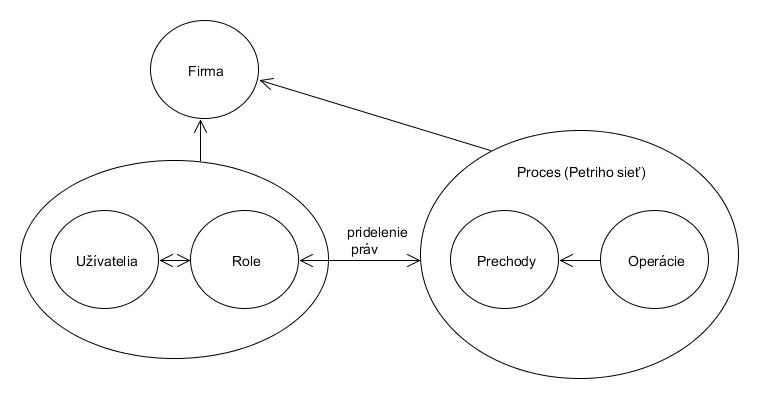
\includegraphics[width=0.9\linewidth]{images/roles_in_petri_model}
	\caption{ Model RBAC v aplikácii}
	\label{fig:model_rbac_v_aplikacii}
\end{figure}

\subsubsection{Priraďovanie používateľov k roliam}
V našej aplikácii nechceme aby bol používateľ viazaný len na jednu firmu. Chceme aby pod rovnakým účtom mohol figurovať vo viacerých firmách, prípadne mal možnosť si založiť vlastnú. Preto je potrebné, aby sa používatelia neviazali len na samotnú rolu. V aplikácii bude väzba používateľa na rolu závislá od konkrétnej firmy. V každej firme bude môcť administrátor, používateľ s právami na riadenie rolí, mať možnosť priradiť používateľa ku konkrétnej roly, ktorá je vo firme zaradená. Samotný používateľ môže byť tým pádom priradený vo viacerých firmách, pričom v každej firme bude mať iné práva.\\

 Na obrázku  \ref{fig:user_to_roles} môžeme vidieť zjednodušený model mapovania právomocí používateľa prostredníctvom systému rolí.
Šedé pozadie v roli znamená, že používateľ je k roli priradený.  V rovnakom procese vidíme, že používateľ, ktorý môže vo firme 1 spustiť prechod 1 , nie je oprávnený vykonať prechod 1 aj vo firme 2, pretože v nej nemá priradenú rolu. Vo firme 2 môže spustiť iba prechod 2.

\begin{figure}[h]
	\centering
	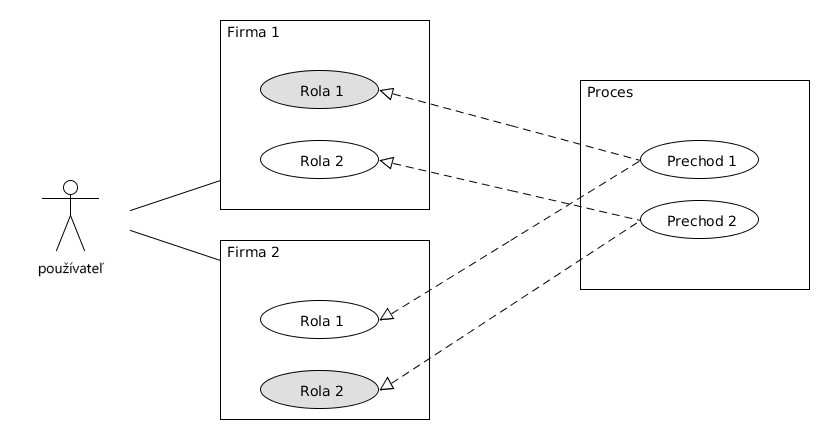
\includegraphics[width=0.9\linewidth]{images/user_to_roles}
	\caption{ Mapovanie používateľov na roly vo firme}
	\label{fig:user_to_roles}
\end{figure}


%\subsection{Riadenie právomocí}	
%Zadefinovali sme si ako sa v aplikácii mapujú používatelia na role. V nasledujúcej časti si bližšie definujeme pravidlá pre spúšťanie prechodov v sieti, rovnako ako aj samotné právomoci ktoré daná rola v procese nadobudne. 



\subsubsection{Priradenie práv k roliam}
Priradenie práv k roliam je definované nepriamo prostredníctvom jednotlivých prechodov. Hlavnou úlohou roly v procese je zadefinovať práva na vytváranie nových prípadov a takisto určiť právomoci na spúšťanie prechodov v procese. Schopnosť spustiť nový prechod je však vymedzená referenciami, návrhom Petriho siete a stave v akom sa tokeny momentálne nachádzajú.  


\begin{figure}[h]
	\centering
	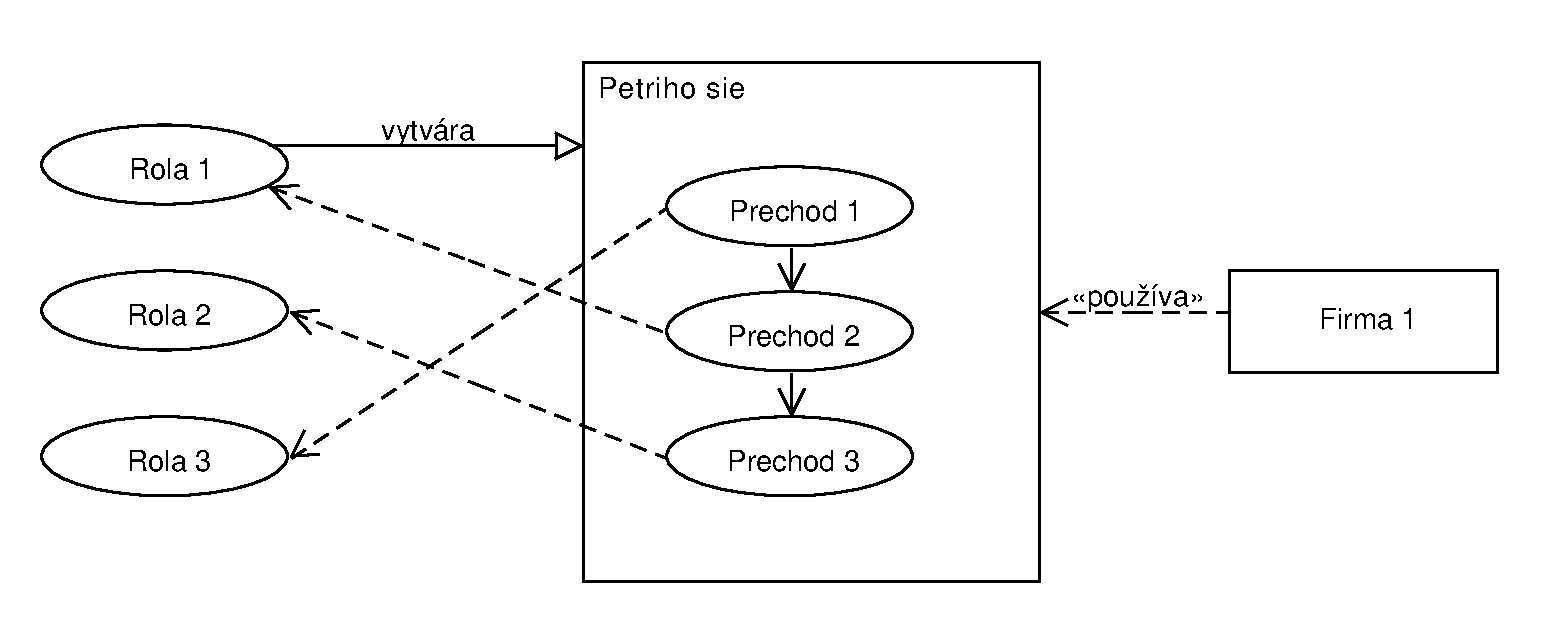
\includegraphics[width=0.9\linewidth]{images/roles_permissions}
	\caption{ Právomoci rolí v sieti }
	\label{fig:roles_permissions}
\end{figure}

\subsubsection{Definovanie prístupových práv ku prechodu}

Osoba môže v jednotlivom prípade spustiť prechod, ak spĺňa nasledovné požiadavky:
\begin{enumerate}
	\item prechod je spustiteľný
	\item osoba je priradená k roli, ktorej daný prechod prináleží
	\item osoba spľňa požiadavky referencie
\end{enumerate}

Spustiteľnosť prechodu je zadefinovaná prostredníctvom Petriho siete. Prechod v sieti je spustiteľný len vtedy, ak každé  miesto vstupujúce do prechodu obsahuje minimálne toľko tokenov, aká je násobnosť hrany medzi daným miestom a prechodom.
V aplikácii máme dva typy referencii: \textbf{referenciu na prechod} a \textbf{referenciu na prvú rolu} .
Ak má prechod nastavenú referenciu na prechod, v databáze sa porovná používateľove id s id používateľa , ktorý spustil referovaný prechod. V prípade, že tieto dáta súhlasia, používateľ je oprávnený spustiť prechod.

Ak má prechod nastavenú referenciu na prvého používateľa, overí sa ,či sa v procese už daná rola nevyskytla. Ak prechod s danou rolou v danom prípade ešte nebol spustený, používateľ je oprávnený tento prechod spustiť. V opačnom prípade je potrebné overiť id používateľa s používateľom ktorý ako prvý spustil prechod s touto rolou. Ak sa zistí zhoda, používateľ môže daný prechod spustiť.



\subsubsection{Operácie nad prechodom}	
Práva, ktoré rola nad prechodom získa sú zadefinované operáciami v konkrétnom prechode. Tieto operácie sa určia pri vytváraní formulára k danému prechodu.  
Vo formulári je možné nastaviť aké dáta budú používateľovi prístupné, či ich bude môcť používateľ iba zobrazovať, alebo aj editovať. Takisto sa definuje, ktoré údaje je potrebné vyplniť, aby mohol používateľ tento prechod dokončiť.

\begin{figure}[h]
	\centering
	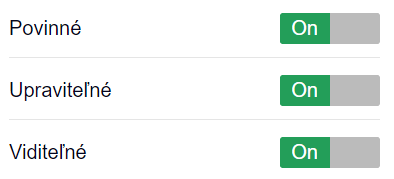
\includegraphics[width=0.4\linewidth]{images/formulare_opravnenia}
	\caption{ Právomoci definované v prechodoch }
	\label{fig:roles_permissions}
\end{figure}





\section{Implementácia}

\subsection{Modul na priraďovanie používateľov k rolám}
Vo WfMS treba zabezpečiť používateľsky ľahko zrozumiteľnú a jednoduchú administráciu rol vo firme. Priraďovanie rol vo firme je realizovaná na dvoch úrovniach: \emph{priradenie jednej role pre viacero používateľov} a \emph{priradenie viacero rolí pre jedného používateľa}. Pre tieto účeli sme vytvorili tabuľku, kde sa zobrazia jednotliví používatelia. Zoznam používateľov sa vytvorí na základe vybranej sekcie. Tieto sekcie delíme podľa filtra na všeobecné - všetci používatelia a takí, ktorí nemajú priradenú rolu a potom sekcia s filtrami podľa rol vo firme - každá rola vo firme obsahuje priradených používateľov. Používateľov je možné usporiadať v každej sekcii podľa ich ID, mena, priezviska alebo e-mailu. Zároveň je možné v každej sekcii na základe týchto rolí vyhľadávať ľudí.

\begin{figure}[h]
	\centering
	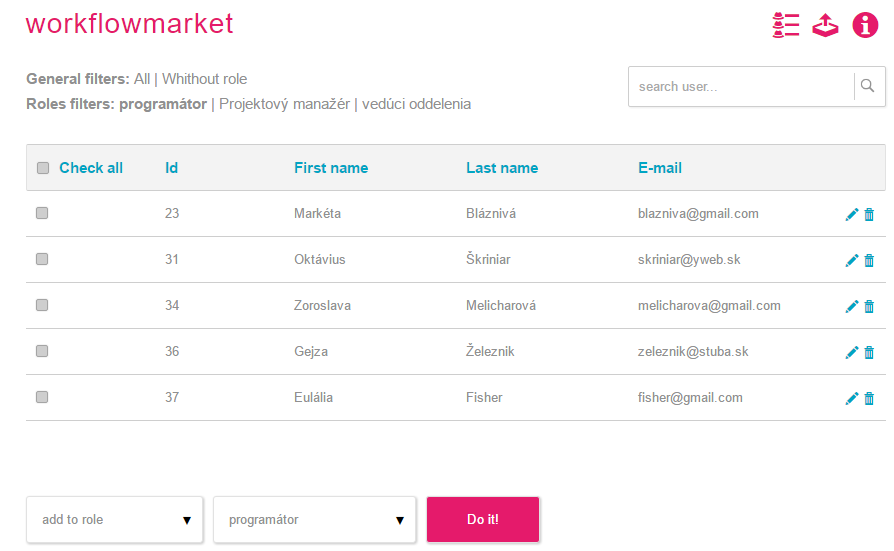
\includegraphics[width=0.9\linewidth]{images/server_roli_screen}
	\caption{ Prideľovanie  }
	\label{fig:server_roli_screen}
\end{figure}

\subsubsection{Priradenie a vyradenie viacerých používateľov z role}
Priradenie a vyradenie viacerých používateľov je založené na dvoch krokoch. Označenie používateľov a následné vybranie žiadanej akcie - add to role (priradenie do role) delete from role (ich odstránenie z role).  

\begin{figure}[h]
	\centering
	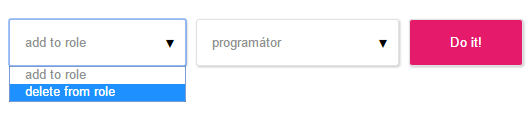
\includegraphics[width=0.5\linewidth]{images/role_actions_screen}
	\caption{ Prideľovanie  }
	\label{fig:server_roli_screen}
\end{figure}

\subsubsection{Priradenie a vyradenie jednotlivca}
Správa samotného používateľa je realizovaná viacerými spôsobmi. Prvý spôsob je rovnaký ako pri správe viacerých používateľov ( označíme ale iba jedného ). Druhý spôsob je detailná správa používateľa. Po kliknutí na podrobnosti konkrétneho používateľa sa zobrazí okno pre konkrétneho používateľa. V ňom sú všetky role do ktorých je možné používateľa priradiť. Jednoduchým kliknutím na tlačítkom sa používateľ priradí alebo odstráni z role. takisto je možné odstrániť používateľa z role priamo z tabuľky kliknutím na ikonu smetného koša.

\begin{figure}[h]
	\centering
	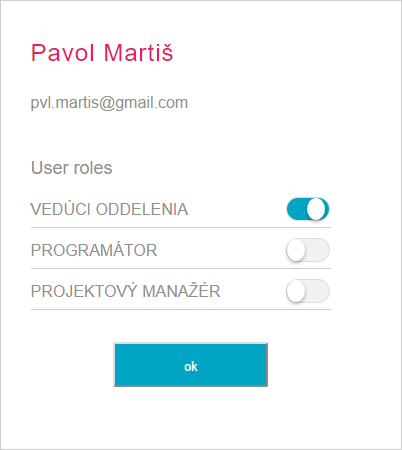
\includegraphics[width=0.5\linewidth]{images/user_detail_screen}
	\caption{ Správa rolí pre konkrétneho používateľa  }
	\label{fig:user_detail_screen}
\end{figure}

\begin{figure}[h]
	\centering
	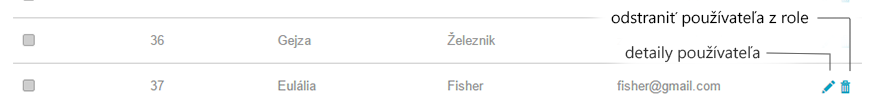
\includegraphics[width=1\linewidth]{images/one_user_screen2}
	\caption{ Vymazanie používateľa priamo z tabuľky  }
	\label{fig:user_detail_screen}
\end{figure}

\subsubsection{Správa rolí vo firme}
Firma musí mať vo svojej štruktúre také role, ktoré používa vo svojich procesoch. Preto sa pri priradení procesu do firmy nahrávajú do firmy roly, ktoré sú v procese využívané (viď. \ref{ukladanie rolí}). Okrem toho sa však dajú vo firme vytvoriť role pred tým ako sa k nemu priradia procesy. Na to slúži administrácia rolí vo firme. Do firmy je tak možné pridať nové role, prípadne odstrániť staré. Pri odstraňovaní rolí sa najprv skontrolujú v databáze, či firma nepoužíva danú rolu v niektorej z jej procesov.

\begin{figure}[h]
	\centering
	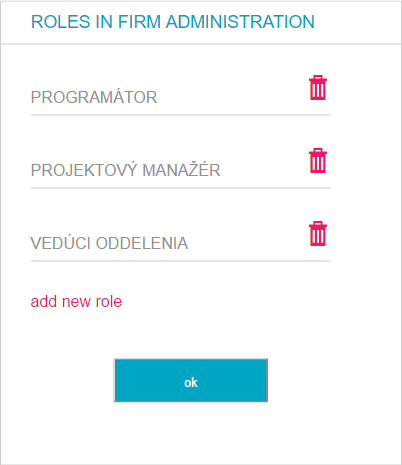
\includegraphics[width=0.5\linewidth]{images/firm_administration_screen}
	\caption{ Administrácia rolí vo firme  }
	\label{fig:Administrácia rolí vo firme}
\end{figure}

\noindent Priradenie rolí do firmy je možné aj za pomoci xml- súboru v podobnej štruktúre:
\begin{lstlisting}[language=XML]
<?xml version="1.0" encoding="UTF-8"?>
<document>
	<roles>
		<role>
			<name>názov role 1</name>
		</role>
		<role>
			<name>názov role 2</name>
		</role>
	</roles>
</document>
\end{lstlisting}


\subsection{Ukladanie rolí a referencii z editoru do databázy}
\label{ukladanie rolí}
Dôležitou časťou serverovej časti rolí je uložiť výstup z \emph{editora rolí}. Celý proces prebieha v nasledovných fázach : 
\begin{enumerate}
	\item vytvorenie a priradenie rolí (v editore)
	\item po tom ako používateľ odošle požiadavku na uloženie do databázy,  sa odošle na server XML súbor spolu s ID procesom  a ID firmy z databázy
	\item na serveri sa najprv vymažú staré dáta (napojenie rolí a referencii na sieť), aby nevznikali problémy pri spätnej úprave
	\item do databázy sa pridajú role 
	\item pridajú sa do databázy spojenia medzi rolou a prechodmi. Uloží sa rola, ktorá môže spustiť prípad a pridajú sa referencie ku prechodom,.
	\item role použité v sieti sa priradia do firmy, z ktorej sa vykonávalo modelovanie
\end{enumerate}

Štruktúra XML súboru a jeho uloženie do databázy:

%\<\!\-\-  \-\-\>
%referencia na prvého používateľa z roly
%<!-- referencia na prechod s id 0 -->
\begin{lstlisting}
<?xml version="1.0" encoding="UTF-8"?>
<document>
<roles>
	<role>  // definovanie role 
		<id>0</id>
		<name>programátor</name>
		<start_case>false</start_case> // určuje či môže rola spustiť prechod
		<transitionId>0</transitionId> 
		<transitionId>1</transitionId>
		<transitionId>2</transitionId>
	</role>
</roles>
<references>
	<reference> // nulová referencia 
		<transitionId>2</transitionId>
		<value>false</value>
	</reference>
	<reference>   // referencia na prechod s id 0
		<transitionId>1</transitionId>
		<value>true</value>
	</reference>
		<reference> 
		<transitionId>0</transitionId>
		<value>0</value>
	</reference>
</references>
</document>
\end{lstlisting}


\subsection{Dátový model}
Dátová časť našej aplikácie je implementovaná v databáze MySQL. Na začiatku je potrebné definovať návrh tabuliek pre uloženie rolí a referencii ku konkrétnej sieti. 

\begin{figure}[h]
	\centering
	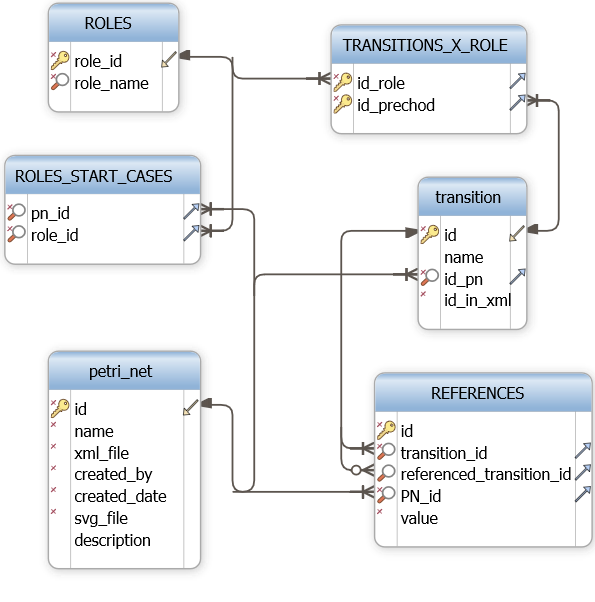
\includegraphics[width=0.7\linewidth]{images/roles_permissions_diagram}
	\caption{ Priradenie právomocí rolám }
	\label{fig:Priradenie právomocí rolám}
\end{figure}
Tabuľka \emph{TRANSITIONS\_X\_ROLE} ukladá právomoci rolí na spustenie konkrétneho prechodu v sieti, tabuľka \emph{ROLES\_START\_CASES}  ukladá rolu, ktorá môže spustiť nový prípad a tabuľka REFERENCES ukladá jednotlivé referencie ku prechodom. Ak má nastavené \emph{value} na false, prechod nemá referenciu. Ak má hodnotu nastavenú na true , skontroluje sa položka \emph{referenced\_transition\_id}.Pokiaľ má tento atribút číselnú hodnotu, referencia odkazuje na prechod s touto id. Pokiaľ má nastavenú hodnotu na NULL, referencia je nastavená na prvého užívateľa z role.



Druhým krokom je návrh databázového modelu, ktorý bude umožňovať konkrétnym používateľom vo firme priradiť rolu. Priradených používateľov vo firme zaznamenávame v tabuľke USERS\_X\_FIRM.
\begin{figure}[H]
	\centering
	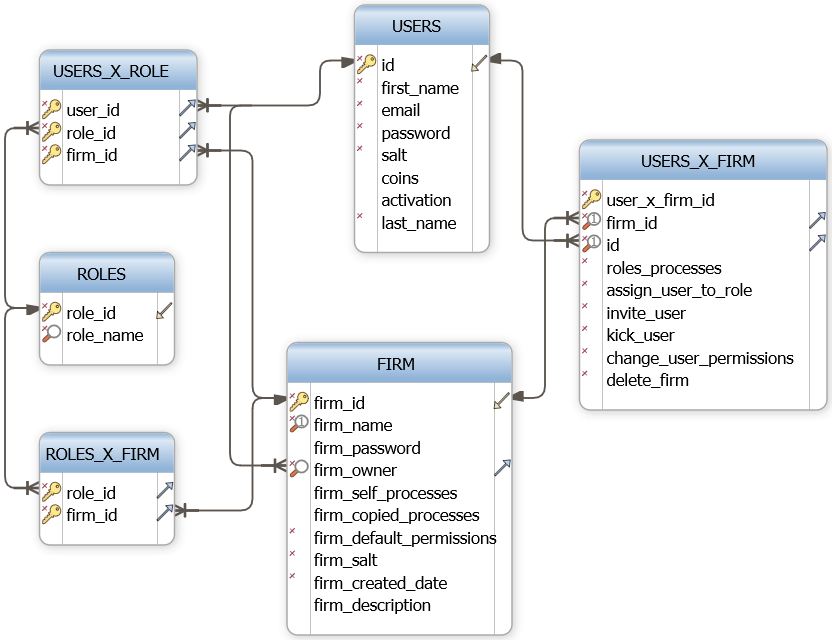
\includegraphics[width=1\linewidth]{images/users_to_roles_diagram}
	\caption{ Priradenie používateľov do rol vo firmách }
	\label{fig:Priradenie používateľov do rol vo firmách}
\end{figure}

\begin{figure}[h]
	\centering
	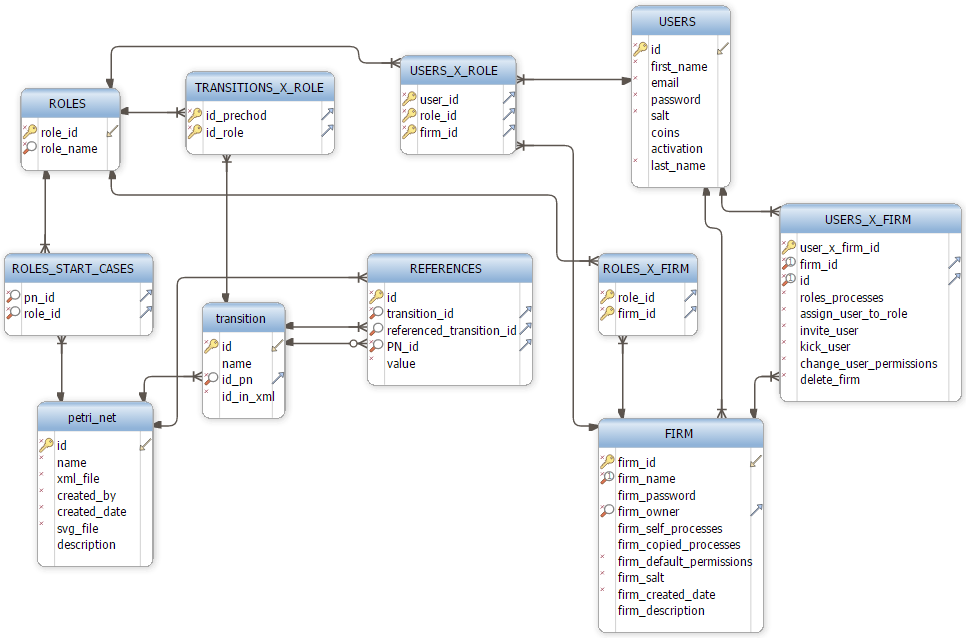
\includegraphics[width=1\linewidth]{images/database_diagram}
	\caption{ Hlavné tabuľky pre prácu s rolami }
	\label{fig:Hlavné tabuľky pre prácu s rolami}
\end{figure}



\begin{figure}[h]
	\centering
	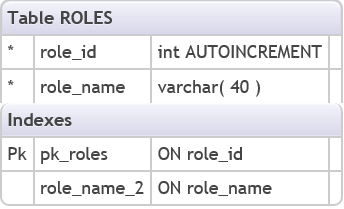
\includegraphics[width=0.4\linewidth]{images/roles_table}
	\caption{ Hlavné tabuľky pre prácu s rolami }
	\label{fig:Hlavné tabuľky pre prácu s rolami}
\end{figure}
Do tabuľky ROLES budeme ukladať role a ich názov. Táto tabuľka má unikátny atribút \emph{názov roly}. Samotná rola sa neviaže na firmu ani na proces. Bolo by tak nežiaduce mať duplicitné záznamy. Vyrieši sa tak aj ukladanie roly do databázy, pretože z XML súboru sa nedá zistiť, či už neexistuje rola rovnaká rola inak ako podľa názvu roly. \\


 V tabuľke TRANSITIONS\_X\_ROLE sa roly viažu  na prechody v Petriho sieti. Každý prechod bude mať v tejto tabuľke presne určené , ktorá roľa ho môže spustiť. \\
 
V tabuľke ROLES\_START\_CASES priradíme k Petriho sieti rolu, ktorá môže spustiť nový prípad.\\
 
V tabuľke REFERENCES definujeme , či má prechod v sieti referenciu. Atribút  \emph{value} typu boolean v tejto tabuľke definuje, či má prechod referenciu. Ak má referenciu, v atribúte \emph{referenced\_transition\_id} sa skontroluje,či obsahuje referenciu na konkrétny prechod. V prípade , že tento atribút má hodnotu NULL, referencia odkazuje na prvý prechod spustený danou rolou v prípade.V prípade , že má nastavenú hodnotu, odkazuje tento atribút na primárny kľúč referencovaného prechodu. \\
  
  
  V tabuľke USERS budú uložený jednotlivý používatelia, ich prihlasovacie a osobné údaje.\\
  
  V tabuľke USERS\_X\_FIRM priraďujeme používateľov ku firmám.\\
  
  V tabuľke USERS\_X\_ROLE priraďujeme používateľom roly v jednotlivých firmách. V tejto tabuľke sme zvolili ako primárny kľúč kombináciu cudzích kľúčov odkazujúcich na id používateľa, role a firmy . 

 
\subsection{Použité technológie}

\section{Overenie riešenia}
TODO